% Created 2025-06-05 Thu 17:54
% Intended LaTeX compiler: pdflatex
\documentclass[10pt,table,dvipsnames,compress]{beamer}
\usepackage[utf8]{inputenc}
\usepackage[T1]{fontenc}
\usepackage{graphicx}
\usepackage{longtable}
\usepackage{wrapfig}
\usepackage{rotating}
\usepackage[normalem]{ulem}
\usepackage{amsmath}
\usepackage{amssymb}
\usepackage{capt-of}
\usepackage{hyperref}
\usetheme{default}
\useinnertheme{rounded}
\useoutertheme[subsection=false]{miniframes}
\date{}
\title{Les forêts tropicales et leur importance pour nos sociétés}
\title[Les forêts tropicales]{Les forêts tropicales et leur importance\\pour nos sociétés}
\definecolor{darkgreen}{RGB}{34,139,34} % vert moyen
\usepackage{float}
\usepackage{lmodern}
\usepackage{pgf}
\usepackage{color}
\usepackage[french,english]{babel}
\definecolor{vertmoyen}{RGB}{51,110,23} % vert moyen
\definecolor{blueFRB}{HTML}{31859c}
\usecolortheme[named=blueFRB]{structure}
\usepackage{tabularx} % varier la largeur du tableau
\usepackage{layout}
\setlength{\LTleft}{-5cm plus 1 fill}
\setlength{\LTright}{-5cm plus 1 fill}
\usepackage{booktabs}
\usepackage{arydshln} %% dashlines for tabular
\newcommand{\logit}{\text{logit}}
\newcommand{\bs}[1]{\boldsymbol{#1}}
\newcommand{\R}{\textnormal{\sffamily\bfseries R}}
\newcommand{\pkg}[1]{{\fontseries{b}\selectfont #1}}
\newcolumntype{C}[1]{>{\centering\arraybackslash}m{#1}}

\setbeamertemplate{footline}[frame number]
\setbeamertemplate{frametitle}{%
\usebeamerfont{frametitle}\insertframetitle%
\vphantom{g} % To avoid fluctuations per frame
\par
\centering 
\includegraphics[width=\textwidth]{figs/Barre_couleur}
}
\beamertemplatenavigationsymbolsempty

% Logo
\newif\ifplacelogo % create a new conditional
\logo{\ifplacelogo
\includegraphics[width=0.4\textwidth]{figs/partners_logos}\fi}

%Call table of contents at the beginning of each section
\AtBeginSection[]{
\placelogotrue
\begin{frame}
\frametitle{Plan de la présentation}
\begin{columns}[c]
\begin{column}{0.5\textwidth}
\tableofcontents[sections=1,currentsection]
\vspace{0.5cm}
\tableofcontents[sections=2,currentsection]
\end{column}
\begin{column}{0.5\textwidth}
\tableofcontents[sections=3,currentsection]
\vspace{0.5cm}
\tableofcontents[sections=4,currentsection]
\end{column}
\end{columns}
\end{frame}
\placelogofalse
}

\hypersetup{
colorlinks=true,
linkcolor=Black,
filecolor=Maroon,
citecolor=Blue,
urlcolor=Maroon}

% Disable monospaced font for URLs
\urlstyle{same}

\hypersetup{
 pdfauthor={Ghislain Vieilledent},
 pdftitle={Les forêts tropicales et leur importance pour nos sociétés},
 pdfkeywords={},
 pdfsubject={},
 pdfcreator={Emacs 30.1 (Org mode 9.7.11)}, 
 pdflang={English}}
\begin{document}

% {
%   % Use background image
%   \usebackgroundtemplate{%
%     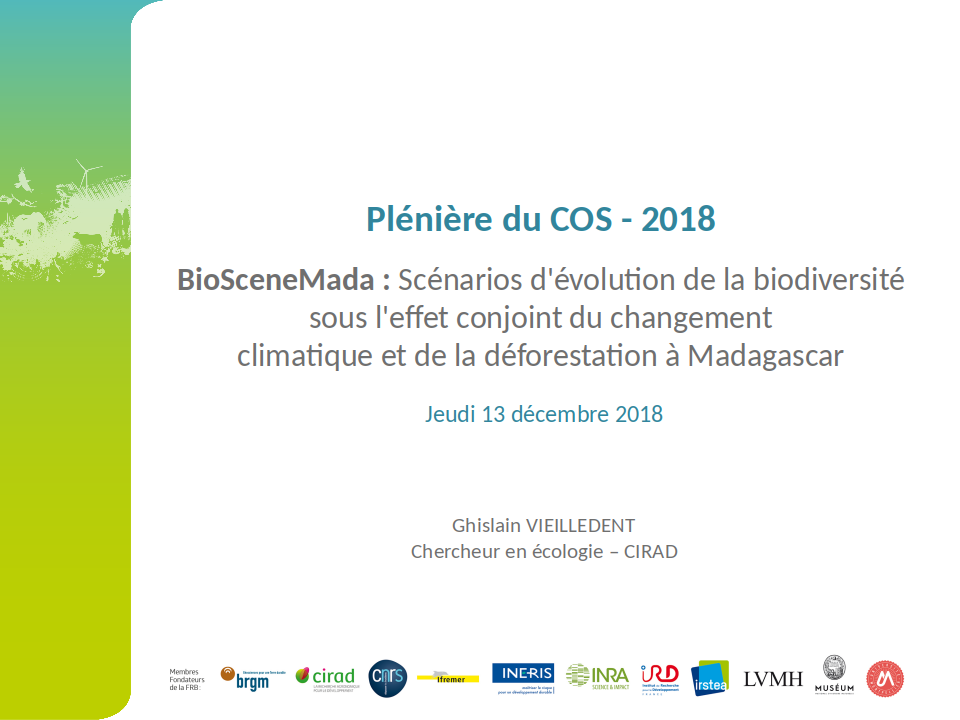
\includegraphics[height=\paperheight,width=\paperwidth]{figs/Masque.png}
%   }
%   \setbeamertemplate{navigation symbols}{}
%   % Remove shadow from block
%   \setbeamertemplate{blocks}[rounded][shadow=false]
%   \begin{frame}[plain]
%   \end{frame}
% }

% Title page
{
  \setbeamertemplate{navigation symbols}{}
  \begin{frame}[plain, noframenumbering]
  \begin{center}
  \small{\textbf{Nouméa, Nouvelle-Calédonie -- 1ère SVT lycée Notre-Dame, Rezé\\Jeudi 06 Juin 2025}}
  \end{center}
  \vspace{-0.5cm}
  \titlepage % Presentation first page
  \vspace{-3cm}
  \begin{center}
    
\includegraphics[width=\textwidth]{figs/Barre_couleur}
    
    \vspace{0.25cm}
    
    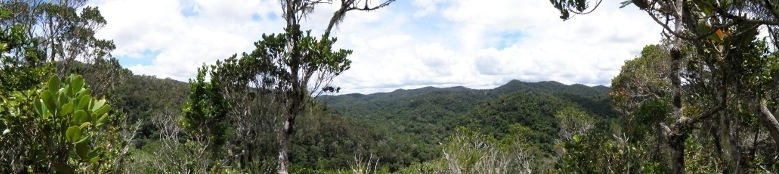
\includegraphics[width=10cm]{figs/Banniere}
    
    \small{Ghislain VIEILLEDENT$^{1}$}
      
    \vspace{0.25cm}
    
    {\scriptsize
      \begin{tabular}{l}
        $[1]$ \textbf{Cirad} UMR AMAP
      \end{tabular}
    }
    
    
\includegraphics[width=0.6\textwidth]{figs/partners_logos}
    
  \end{center}
  \end{frame}
}

% %%%%%%%%%%%%%%%%%%%%%%%%%%%%%%%%%%%%%%%%%%%%%%%%%%%%%%%%%%%%%%%%

% \placelogotrue
% \begin{frame}
%   \frametitle{Outline}
%   \begin{columns}[c]
%     \begin{column}{0.5\textwidth}
%       \tableofcontents[sections=1]
%       \vspace{0.5cm}
%       \tableofcontents[sections=2]
%     \end{column}
%     \begin{column}{0.5\textwidth}
%         \tableofcontents[sections=3]
%         \vspace{0.5cm}
%         \tableofcontents[sections=4]
%     \end{column}
%   \end{columns}
% \end{frame}
% \placelogofalse
\section{Les forêts tropicales}
\label{sec:orgb955b1e}

\subsection{Qu'est-ce qu'une forêt tropicale ?}
\label{sec:orgcadce0c}

\begin{frame}[label={sec:org6c367b3}]{Qu'est-ce qu'une forêt ?}
\begin{center}
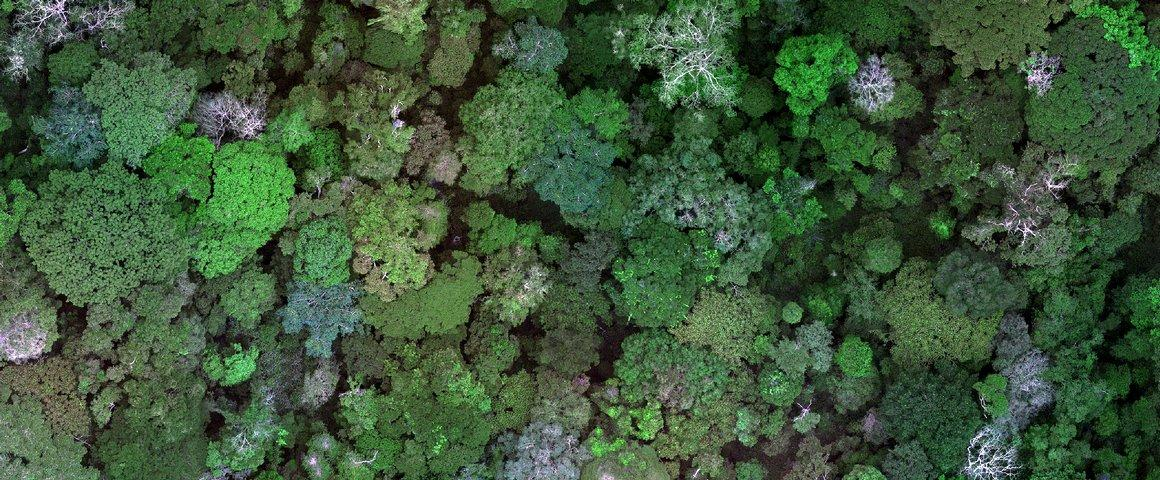
\includegraphics[width=\textwidth]{figs/vue-drone-foret-tropicale-2.jpg}
\end{center}

\begin{itemize}
\item Forêt: ensemble d'arbres de plus de 5 m de haut et de 0.5 ha (définition de la FAO).
\end{itemize}
\end{frame}
\begin{frame}[label={sec:org91eda36}]{Qu'est-ce qu'une forêt tropicale ?}
\begin{center}
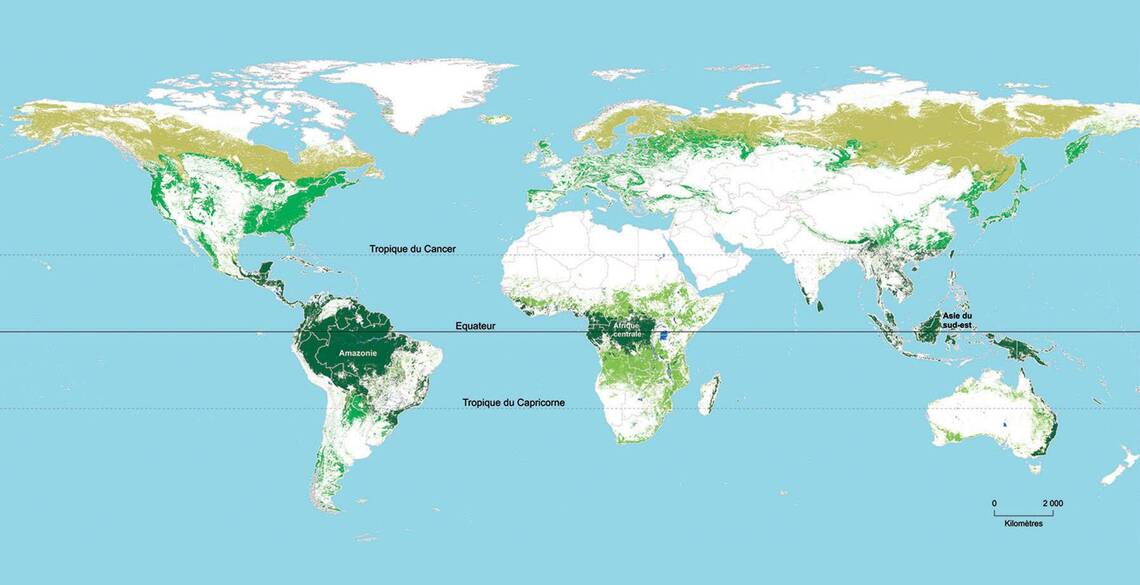
\includegraphics[width=\textwidth]{figs/carte-des-forets-tropicales.jpg}
\end{center}

\begin{itemize}
\item Forêt tropicale: qui se trouve entre les tropiques. \textpm{}23\textsuperscript{\textdegree{}} au nord ou au sud de l'équateur.
\end{itemize}
\end{frame}
\begin{frame}[label={sec:org4324910}]{Qu'est-ce qu'une forêt tropicale ?}
\begin{columns}
\begin{column}{0.3\columnwidth}
\begin{center}
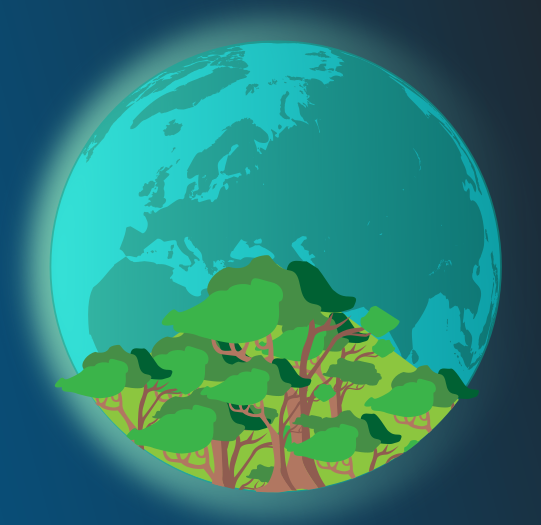
\includegraphics[width=\textwidth]{figs/forest-one-third-of-earth-land.png}
\end{center}
Les forêts couvrent 1/3 de la surface des terres émergées.
\end{column}
\begin{column}{0.7\columnwidth}
\begin{center}
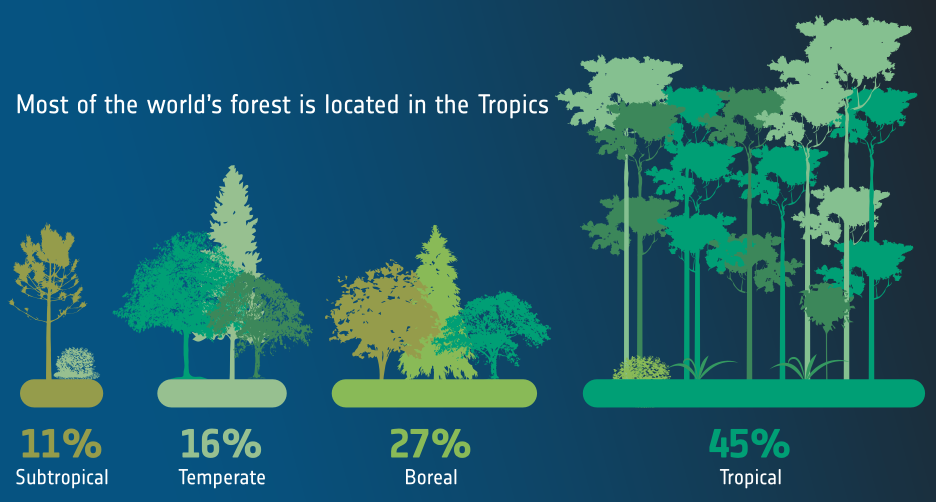
\includegraphics[width=\textwidth]{figs/45-percent-of-forest-cover-in-the-tropics.png}
\end{center}
\begin{itemize}
\item Les forêts tropicales représentent 45\% des forêts du monde.
\item Petit calcul: (1/3 \texttimes{} 0.45) \(\rightarrow\) forêts tropicales couvrent \(\approx\)15\% des terres.
\end{itemize}
\end{column}
\end{columns}
\end{frame}
\subsection{Un réservoir de biodiversité}
\label{sec:orgb3057ba}

\begin{frame}[label={sec:orga6b6524}]{Un réservoir de biodiversité}
\begin{center}
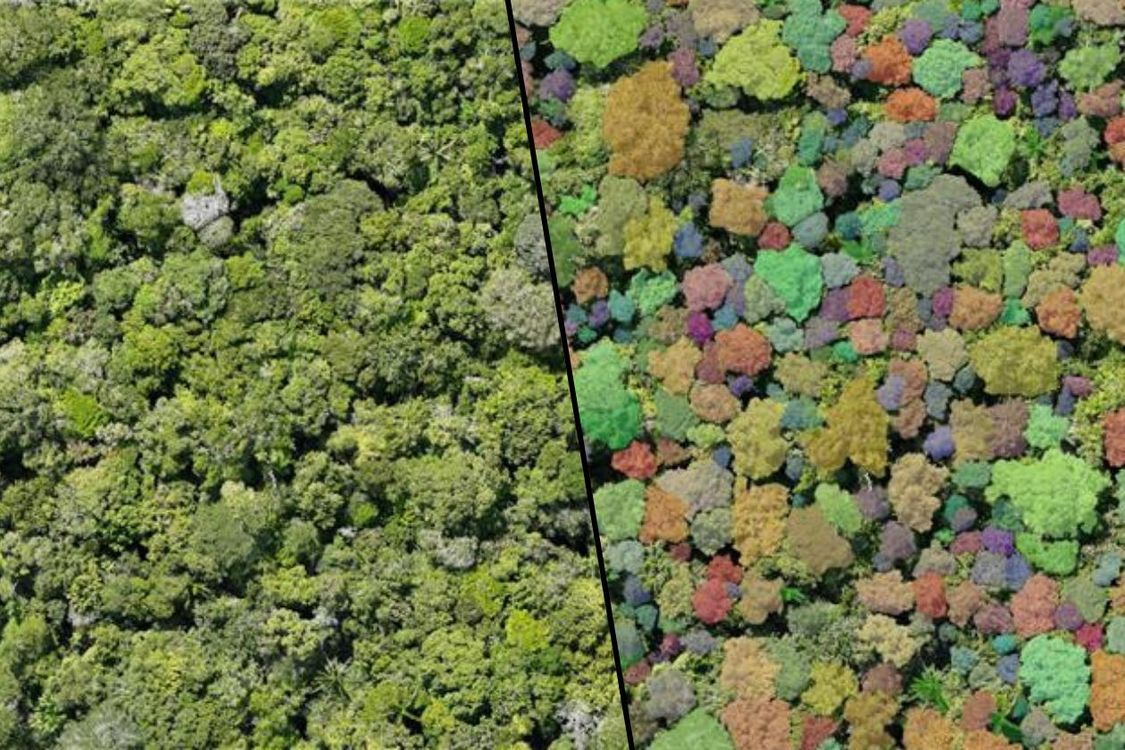
\includegraphics[width=0.8\textwidth]{figs/vue-drone-foret-tropicale.jpg}
\end{center}

Plus de 100 espèces d'arbres à l'hectare en forêt tropicale.
\end{frame}
\begin{frame}[label={sec:org8633800}]{Un réservoir de biodiversité}
\begin{columns}
\begin{column}{0.5\columnwidth}
\begin{center}
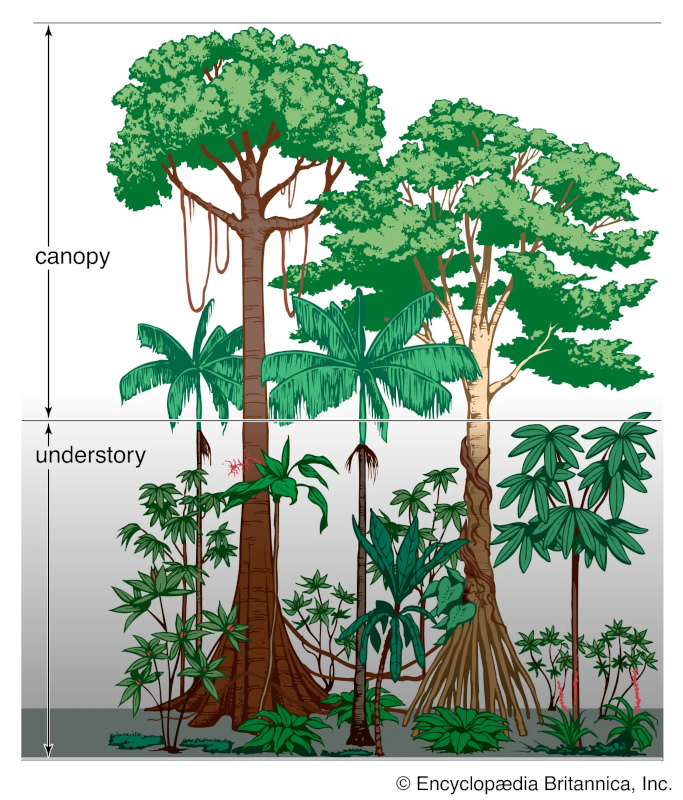
\includegraphics[width=\textwidth]{figs/vegetation-profile-rainforest.png}
\end{center}
\end{column}
\begin{column}{0.5\columnwidth}
\begin{center}
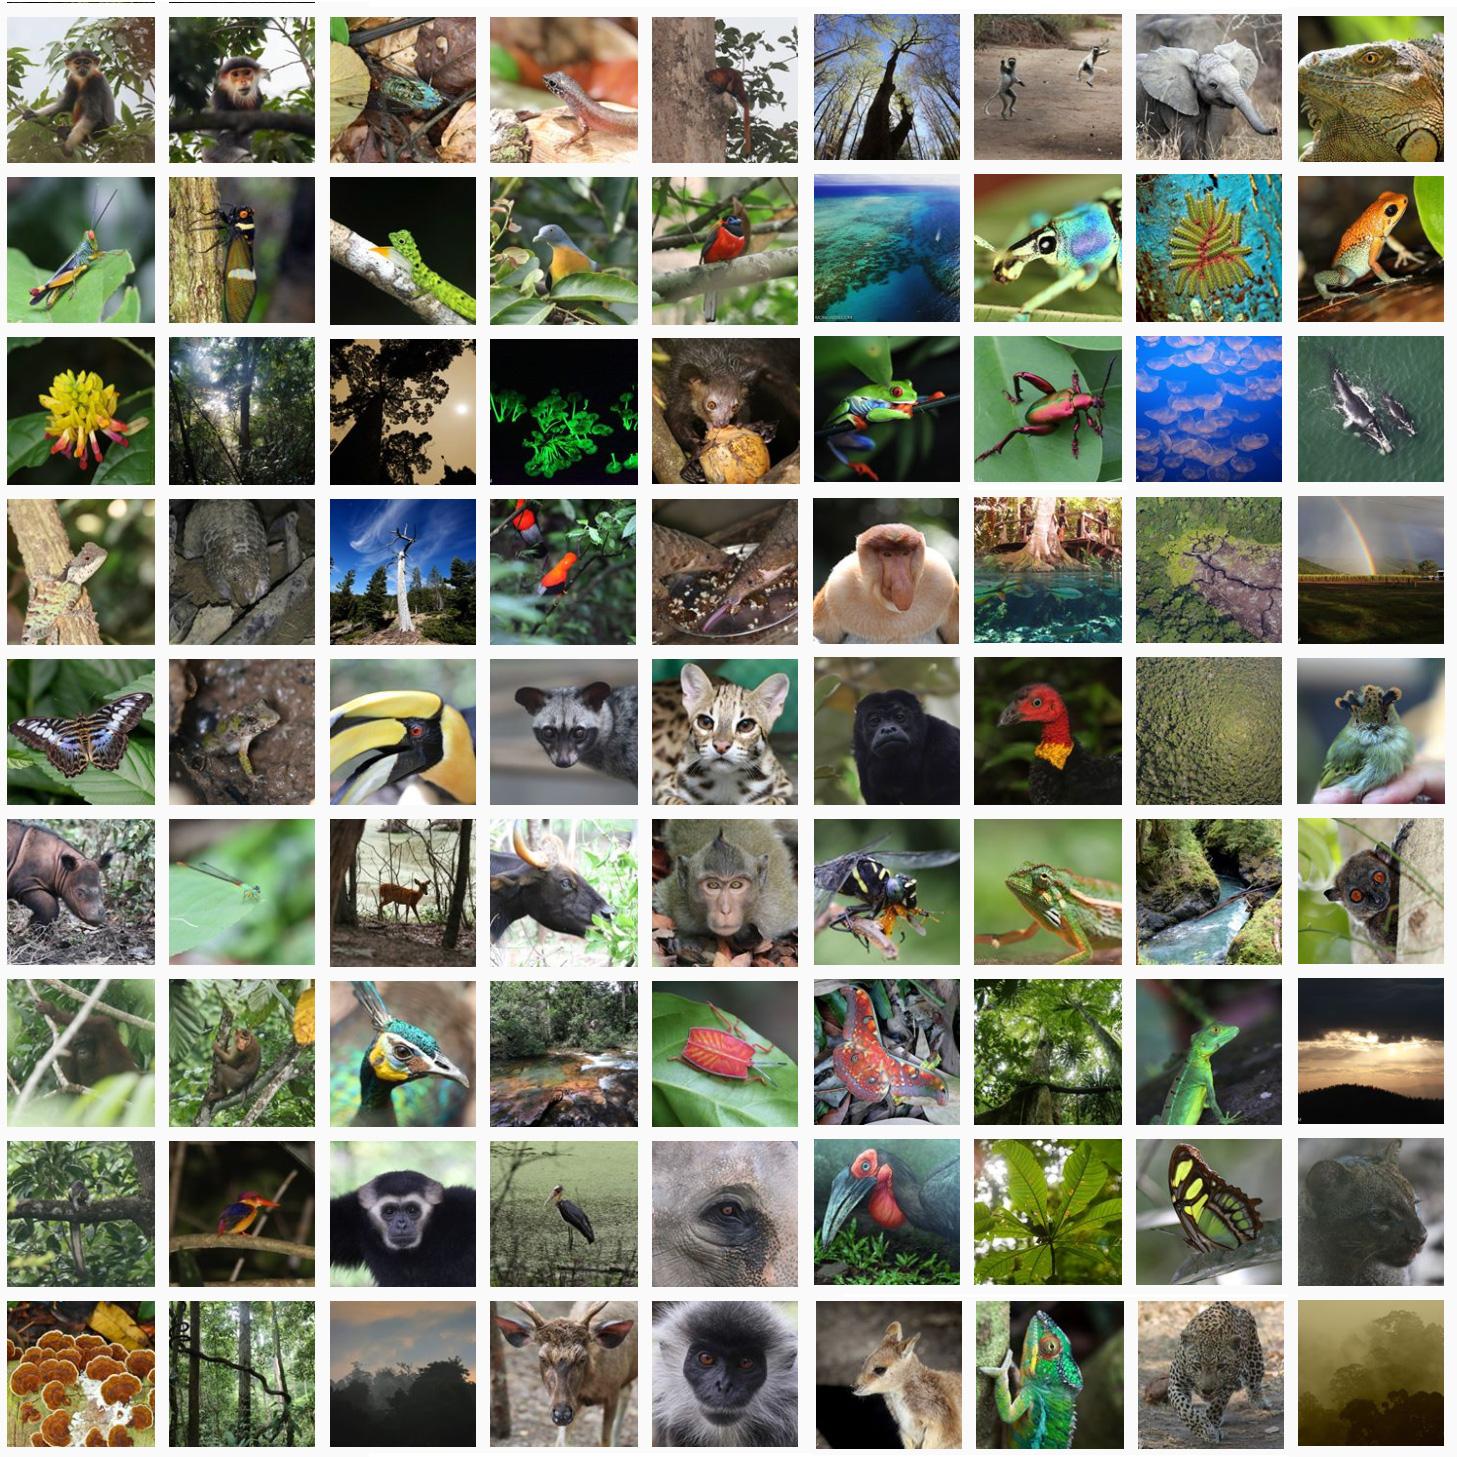
\includegraphics[width=\textwidth]{figs/biodiversity-in-tropical-forests.jpg}
\end{center}
\end{column}
\end{columns}
Un habitat en trois dimensions abritant une multitude d'espèces animales et végétales.
\end{frame}
\begin{frame}[label={sec:org8f8c544}]{Un réservoir de biodiversité}
\begin{center}
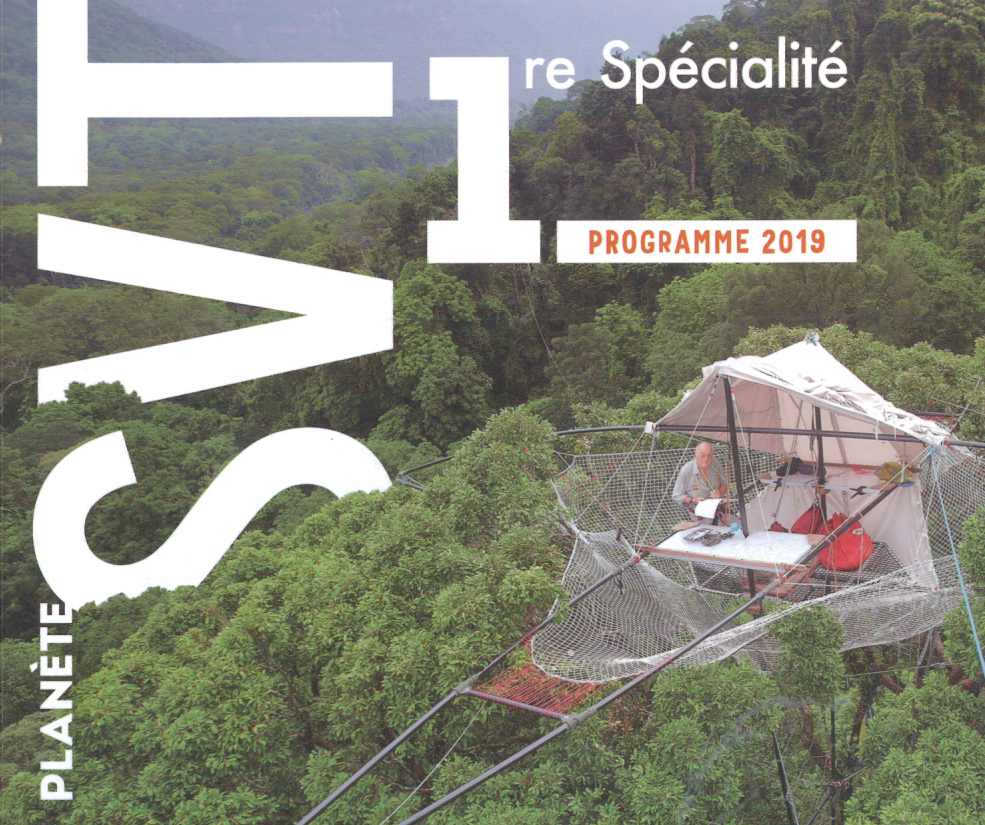
\includegraphics[width=0.7\textwidth]{figs/planete-svt.png}
\end{center}

Le radeau des cimes inventé par Francis Hallé, chercheur et botaniste à l'Université de Montpellier.
\end{frame}
\begin{frame}[label={sec:org5f715ad}]{Un réservoir de biodiversité}
\begin{center}
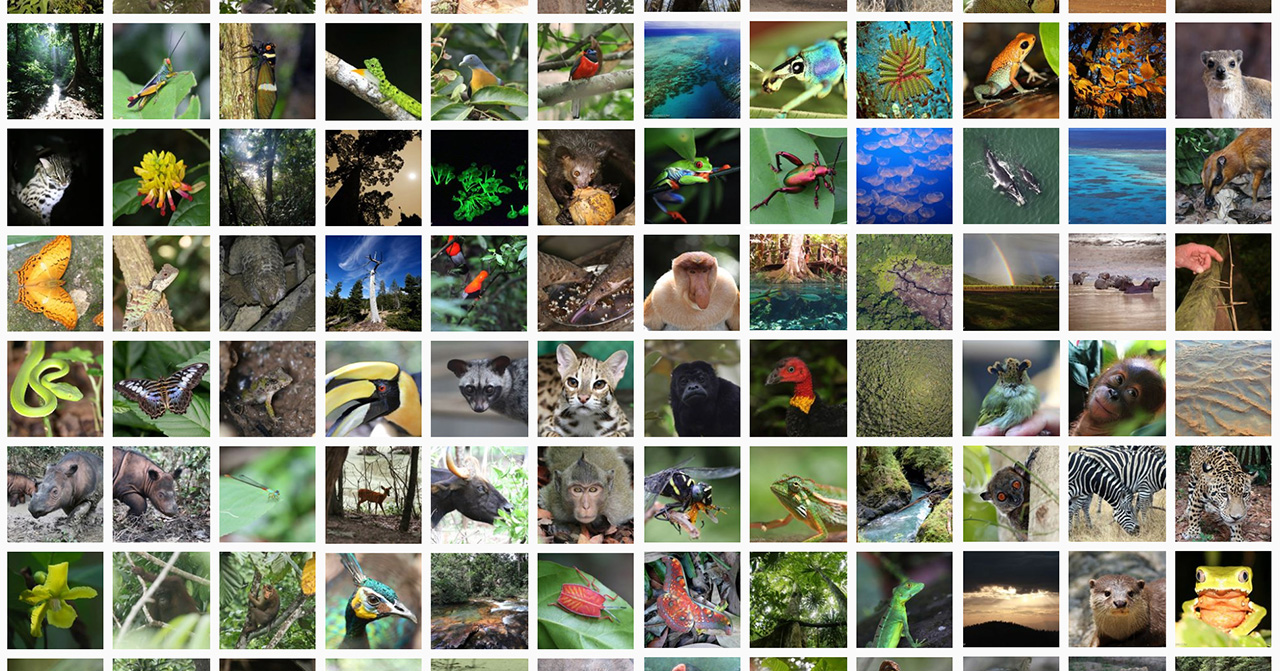
\includegraphics[width=0.8\textwidth]{figs/biodiversity-in-tropical-forests-2.jpg}
\end{center}

Les forêts tropicales ne représentent que 15\% des terres émergées mais elles abritent >50\% des espèces vivant sur ces terres.
\end{frame}
\begin{frame}[label={sec:orga92a8c0}]{Importance de la biodiversité}
\begin{center}
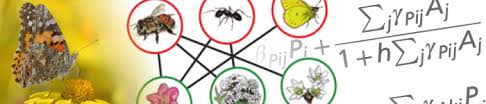
\includegraphics[width=0.8\textwidth]{figs/biodiversity-network.jpg}
\end{center}

\begin{itemize}
\item Les espèces interagissent entre elles et dépendent les unes des autres.
\item Si les espèces disparaissent, l'écosystème peut s'effondrer et ne plus fournir de services (cf. plus bas).
\item Analogie avec un avion: on pert un boulon ça peut passer mais si on pert tous les boulons\ldots{}
\item Actuellement, perte d'un grand nombre d'espèces à un rythme rapide (cf. crise de l'Anthropocène, 6\textsuperscript{ième} extinction de masse).
\end{itemize}
\end{frame}
\section{Les services rendus par les forêts tropicales}
\label{sec:org02191cf}

\subsection{Le stockage du carbone}
\label{sec:org846051b}

\begin{frame}[label={sec:org3a077c1}]{Le stockage de carbone (ou CO2)}
\begin{center}
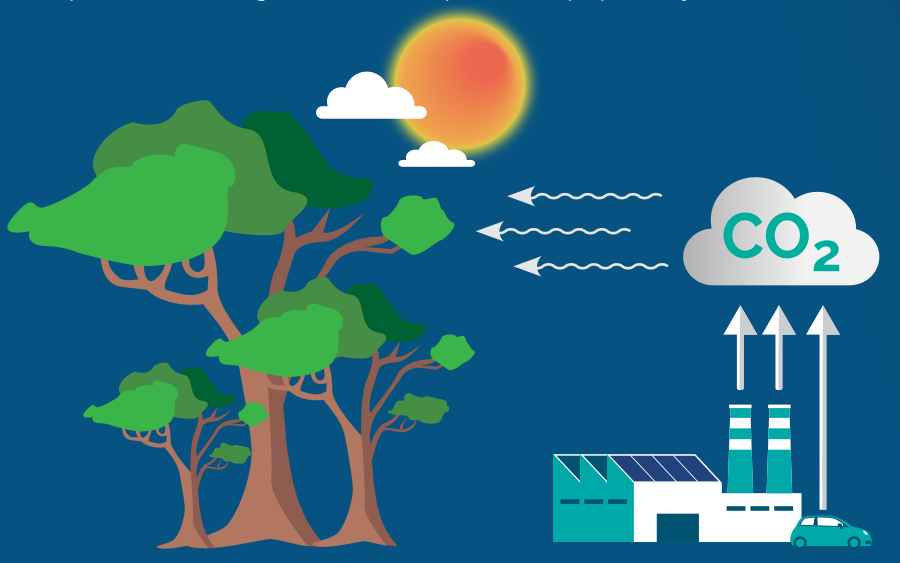
\includegraphics[width=0.6\textwidth]{figs/carbon-sequestration-by-forests.png}
\end{center}

\begin{itemize}
\item Via la photosynthèse.
\item Les forêts absorbent environ 20\% des émissions de CO2 associées aux activités humaines. Elles limitent le changement climatique.
\item En forêt tropicale, un gros arbre séquestre plusieurs tonnes de carbone. 70\% des stocks de carbone sur les terres se situent en forêt tropicale.
\end{itemize}
\end{frame}
\subsection{Les forêts et le cycle de l'eau}
\label{sec:org7b66954}

\begin{frame}[label={sec:org66bc345}]{Les forêts et le cycle de l'eau}
\begin{center}
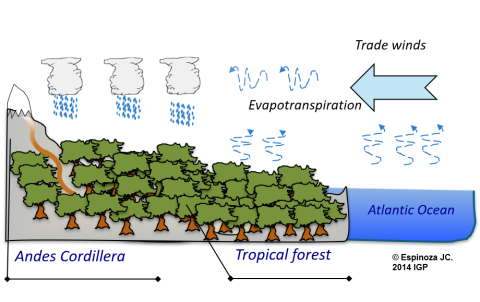
\includegraphics[width=0.7\textwidth]{figs/evapotranspiration-amazonie.png}
\end{center}

\begin{itemize}
\item Les forêts contribuent à la formation des nuages et au régime des précipitations à une échelle régionale via l'évapotranspiration.
\item Les forêts par interception de la pluie, stockage et filtration de l'eau dans les sols forestiers permettent un apport d'eau régulier et de qualité aux populations locales.
\end{itemize}
\end{frame}
\subsection{Les ressources forestières}
\label{sec:org0097c36}

\begin{frame}[label={sec:orga346c2b}]{Les ressources forestières}
\begin{columns}
\begin{column}{0.5\columnwidth}
\begin{center}
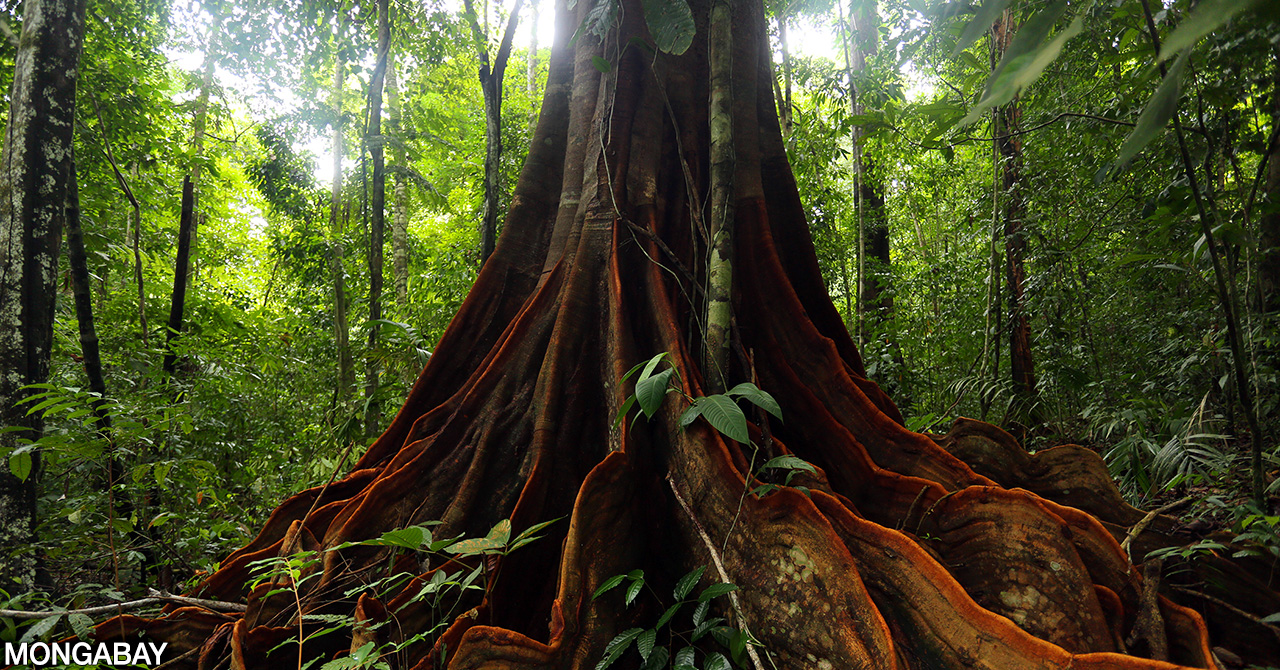
\includegraphics[width=\textwidth]{figs/costa_rica_osa_0077_1280x670.jpg}
\end{center}
\end{column}
\begin{column}{0.5\columnwidth}
\begin{center}
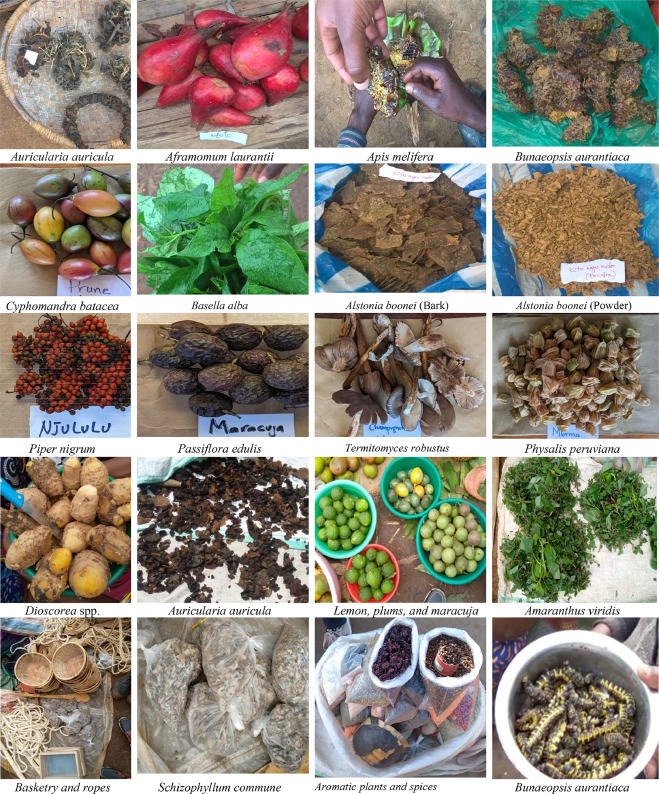
\includegraphics[width=0.6\textwidth]{figs/cueillette.jpg}
\end{center}
\end{column}
\end{columns}
\begin{itemize}
\item Ressources en bois.
\item Ressources alimentaires: chasse, cueillette, miel.
\item Soins: plantes médicinales et pharmacopée traditionnelle.
\item 1.6 milliard d'êtres humains (nous sommes 8 milliards en 2025) dépendent \textbf{directement} des forêts pour leur survie quotidienne.
\end{itemize}
\end{frame}
\section{L'homme destructeur ou protecteur des forêts}
\label{sec:org46d7217}

\subsection{La déforestation}
\label{sec:orgb42c0fa}

\begin{frame}[label={sec:orga2e073e}]{La déforestation}
\begin{center}
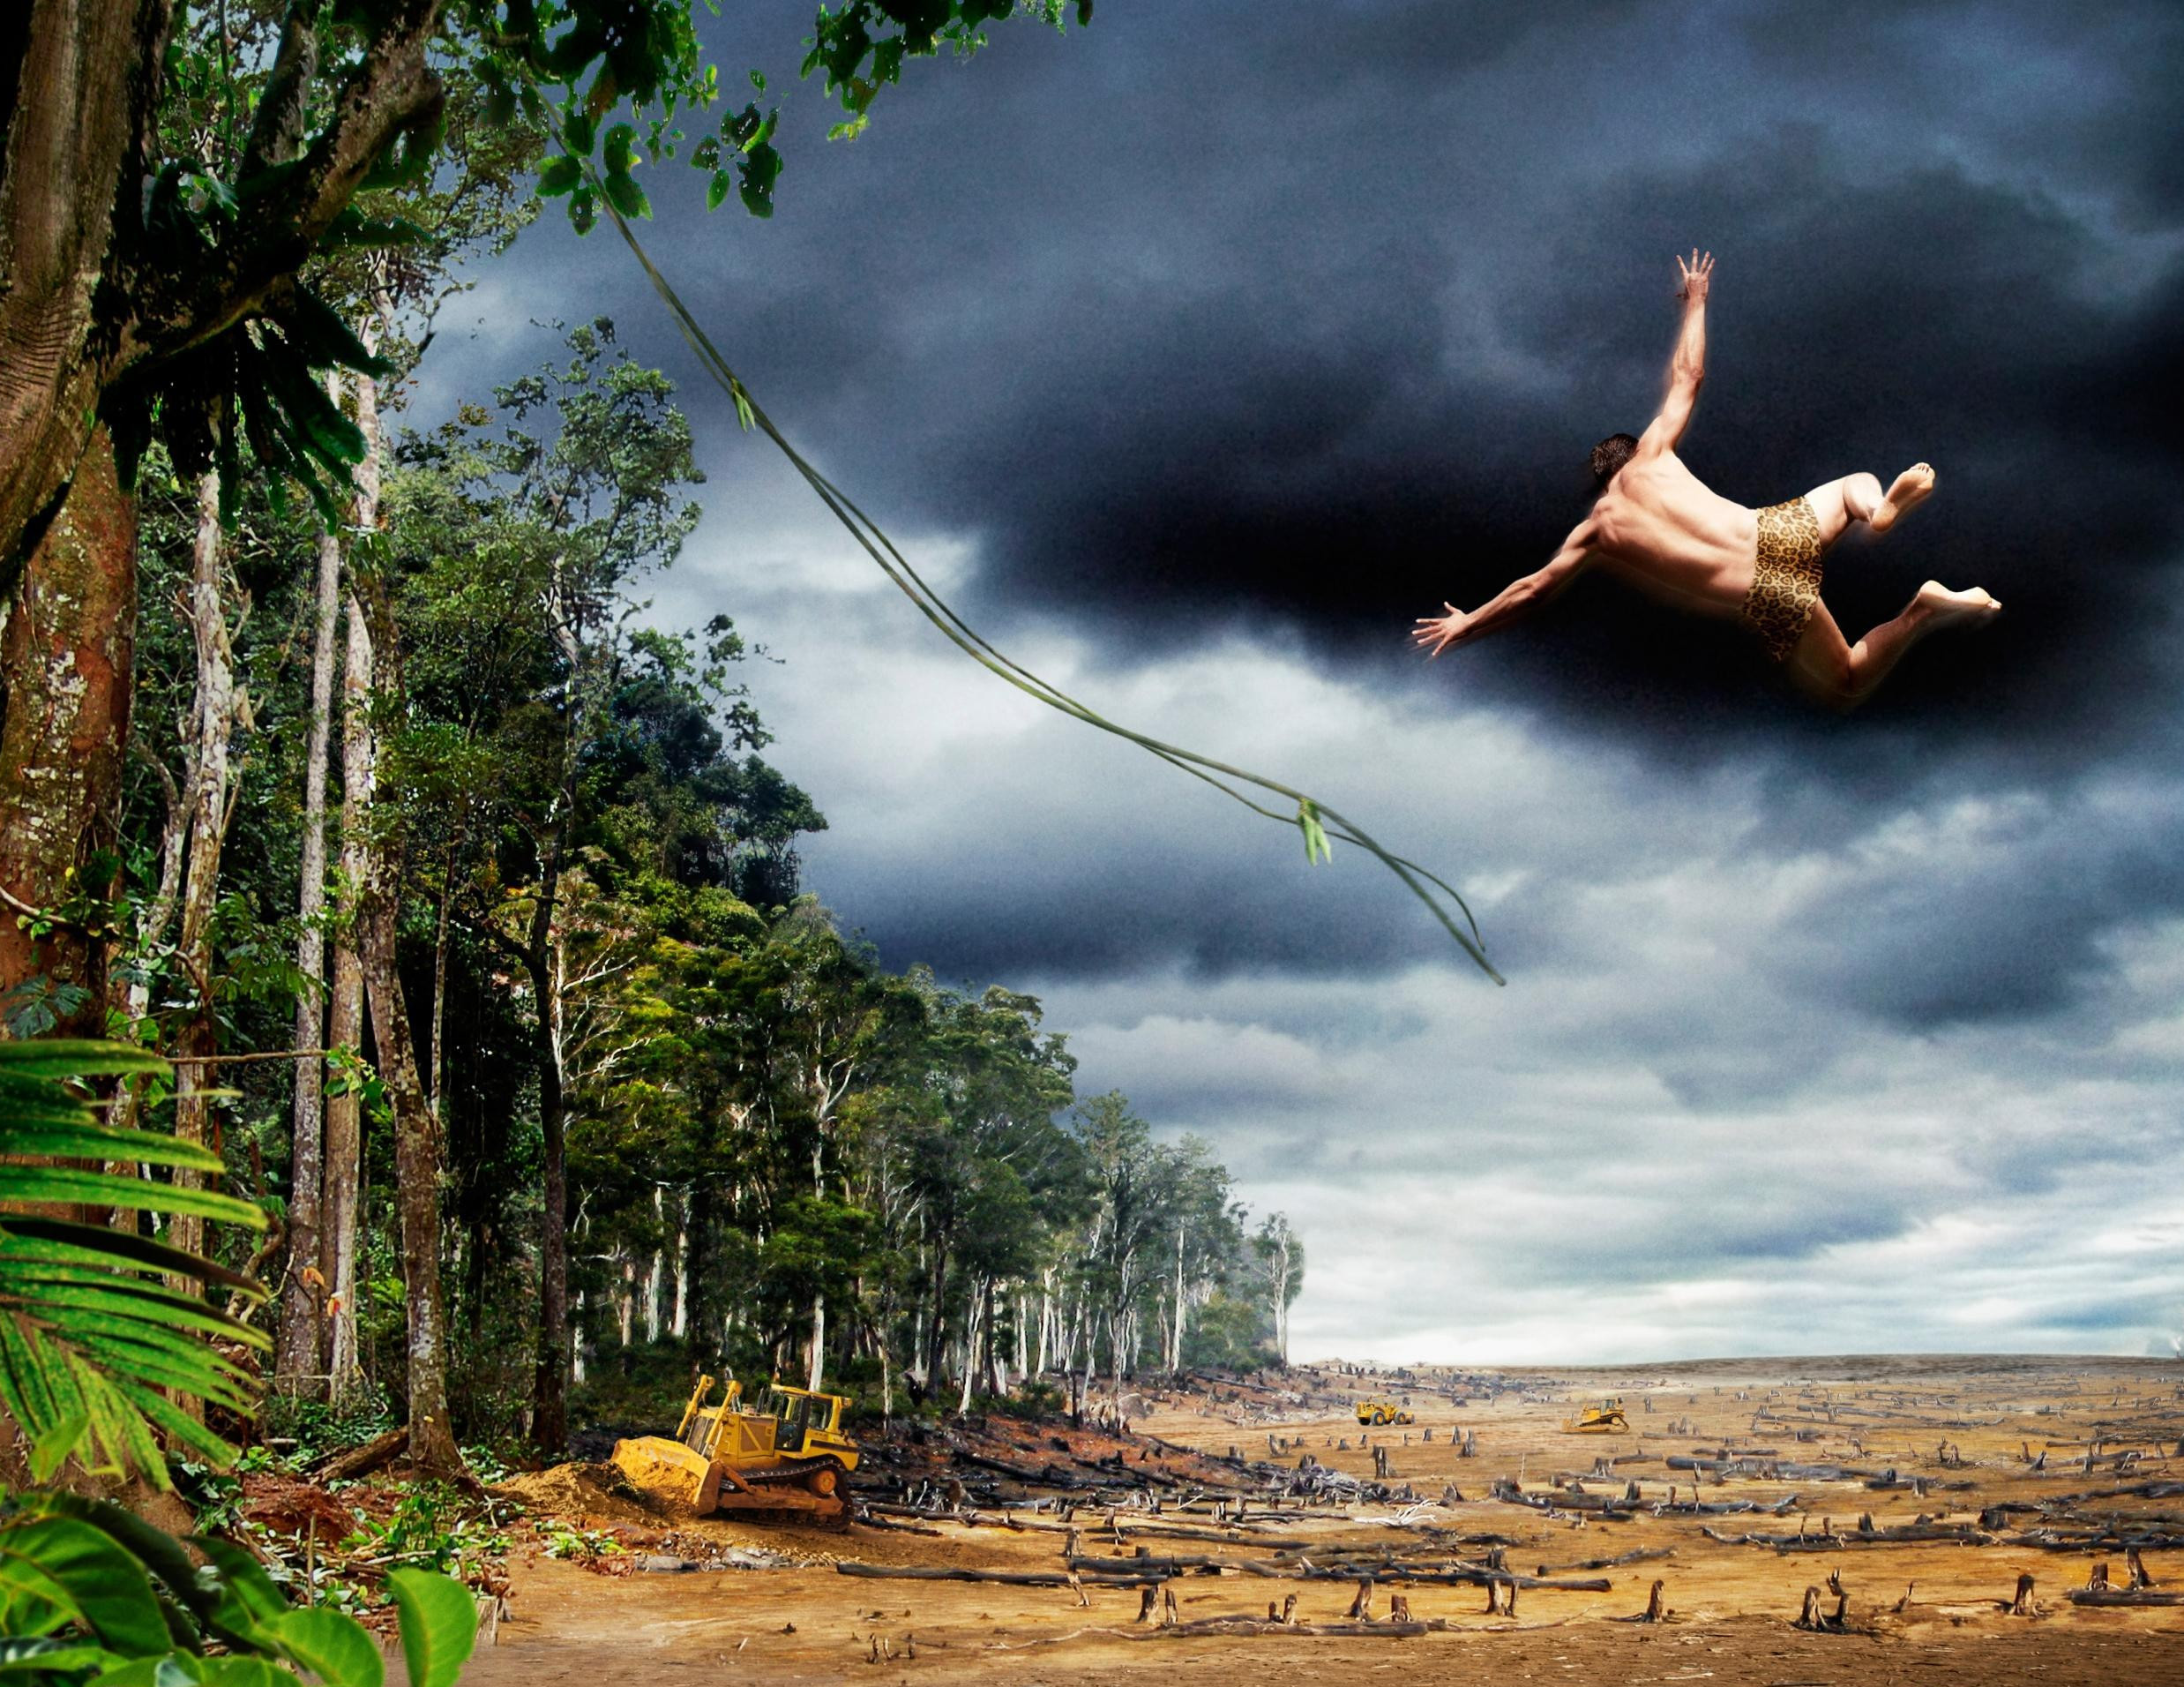
\includegraphics[width=0.6\textwidth]{figs/tarzan.jpg}
\end{center}

\begin{itemize}
\item 10 millions d'hectares par an sont déforestés (1/5 de la France tous les ans, 1 ha \(\approx\) 1 terrain de foot).
\item En conséquence: perte de biodiversité, émissions de CO2, érosion des sols et désertification.
\end{itemize}
\end{frame}
\begin{frame}[label={sec:org8045215}]{Les causes de la déforestation}
\begin{figure}[htbp]
\centering
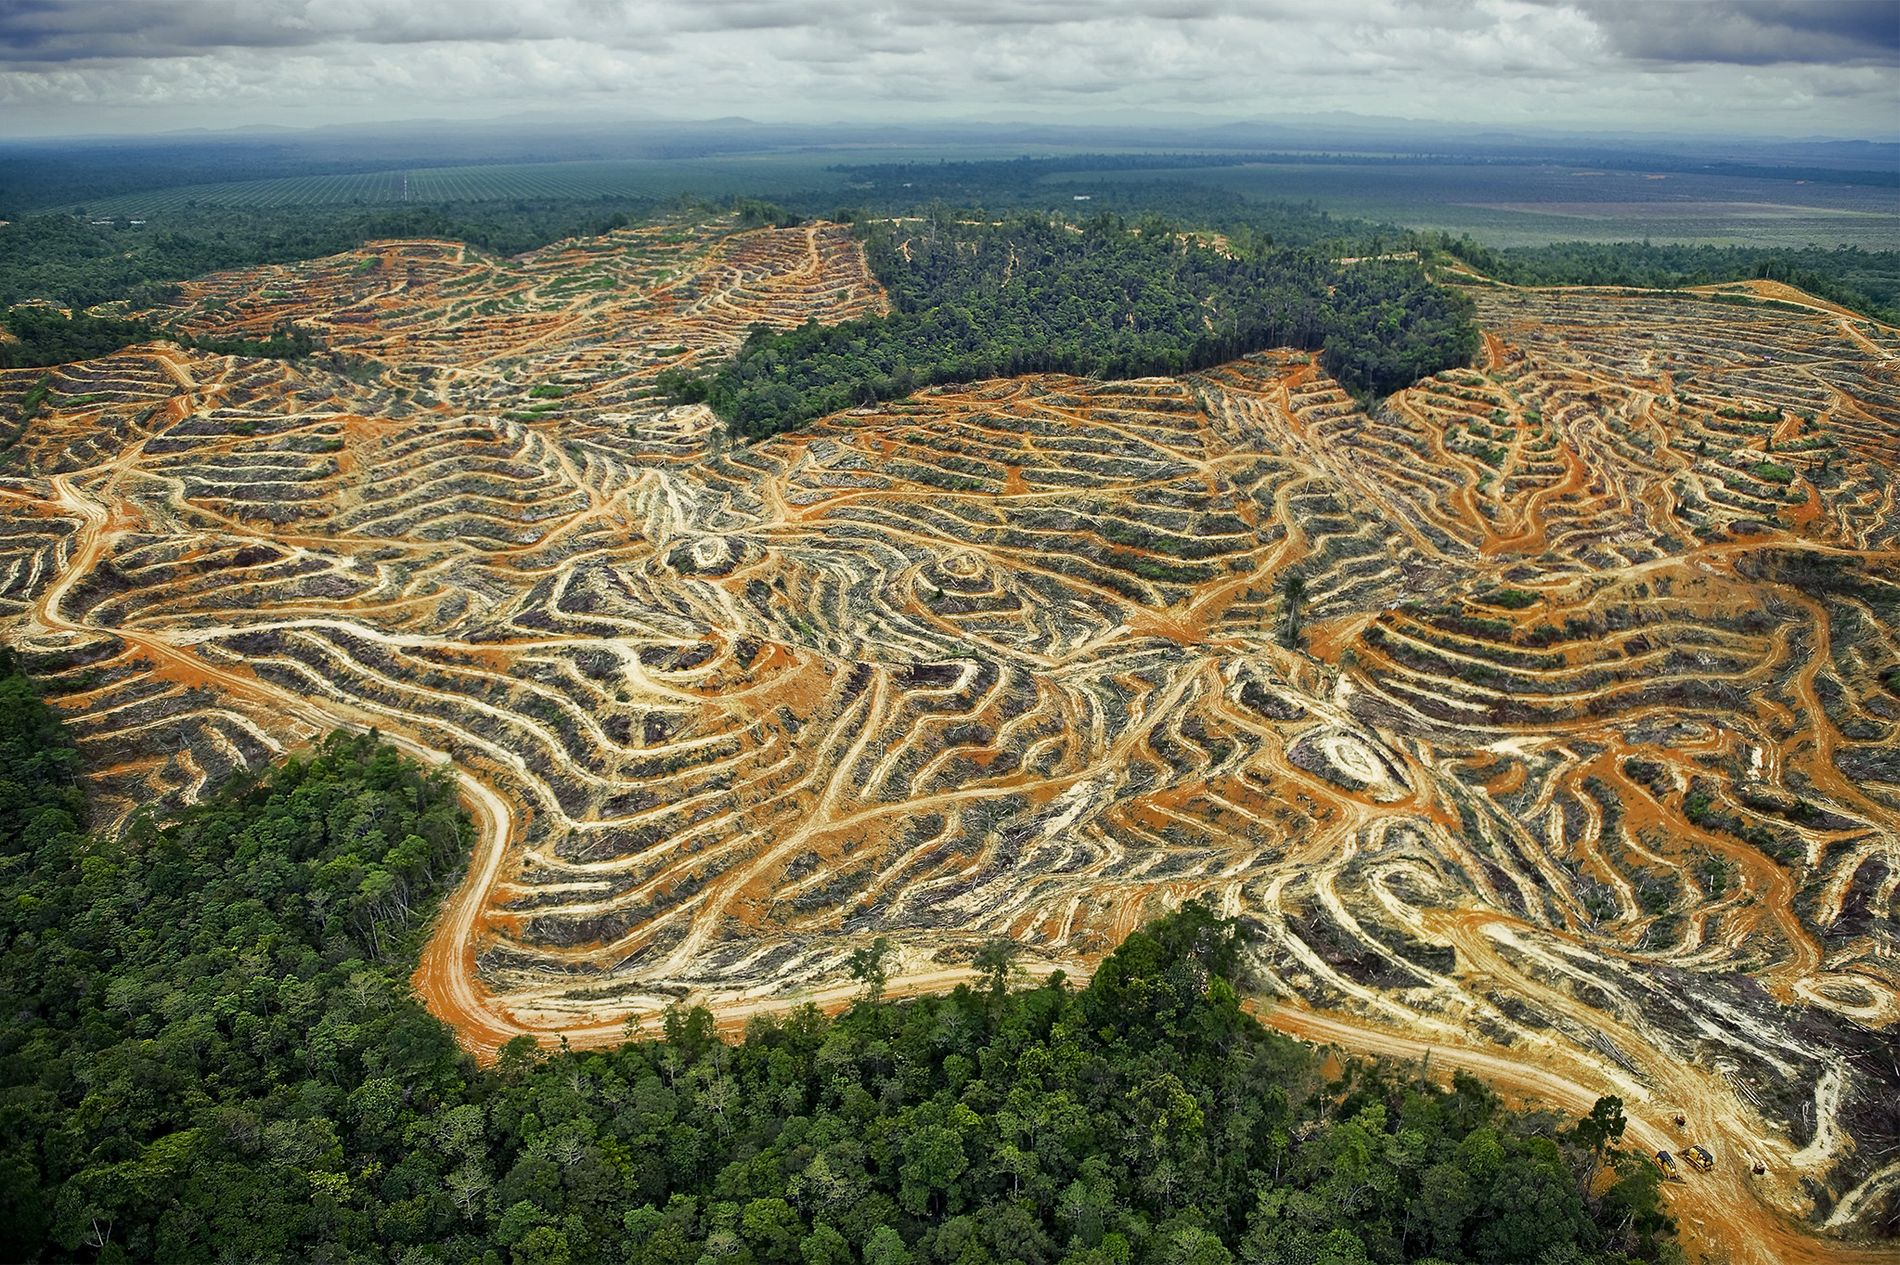
\includegraphics[width=0.6\textwidth]{figs/plantations-huile-de-palme.jpg}
\caption{Déforestation pour la plantation d'huile de palme à Bornéo (Indonésie).}
\end{figure}

\begin{itemize}
\item Agriculture: soja, café, cacao, arachide, pâturages.
\item Plantations: palmiers à huile, hévéa, acacia pour la pâte à papier.
\item Activités minières.
\end{itemize}
\end{frame}
\subsection{Le changement climatique}
\label{sec:org5b5b416}

\begin{frame}[label={sec:org8071374}]{Le changement climatique}
\begin{center}
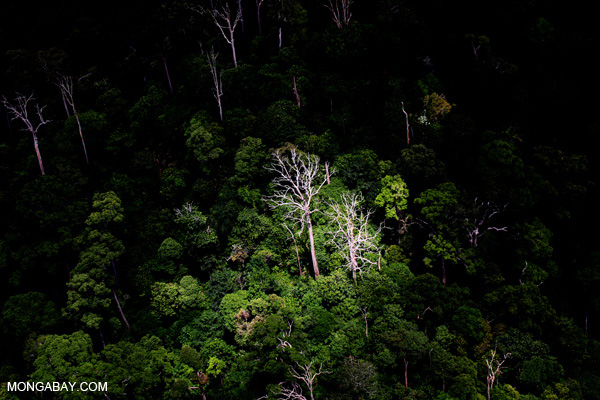
\includegraphics[width=0.6\textwidth]{figs/sabah_1899-forest-dieback.jpg}
\end{center}

\begin{itemize}
\item Mortalité en masse de certaines espèces qui ne résistent pas à l'augmentation des températures.
\item Augmentation de la fréquence des feux et des cyclones qui détruisent la forêt.
\item On ne sait pas dire aujourd'hui si les forêts tropicales pourront résister au changement climatique. Cela reste un sujet de recherche.
\end{itemize}
\end{frame}
\subsection{La conservation des forêts}
\label{sec:org166304c}

\begin{frame}[label={sec:orgef8475d}]{Les aires naturelles protégées}
\begin{center}
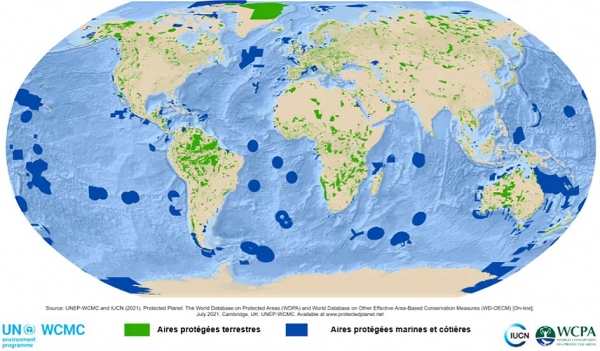
\includegraphics[width=0.8\textwidth]{figs/carte-aires-protegees.jpg}
\end{center}

\begin{itemize}
\item Protection de la nature dans des zones d'intérêt identifiées.
\item Objectif 30/30: protéger 30\% de la planète à l'horizon 2030.
\item Décidé en 2022 à la COP15 de la Convention pour la diversité biologique.
\item Actuellement: 8\% pour les mers et 16.8\% des terres.
\end{itemize}
\end{frame}
\begin{frame}[label={sec:org7bb747e}]{La liste rouge des espèces et des écosystèmes}
\begin{columns}
\begin{column}{0.5\columnwidth}
\begin{center}

\includegraphics[width=\textwidth]{figs/iucn-logo.jpg}
\end{center}
\end{column}
\begin{column}{0.5\columnwidth}
\begin{center}
\includegraphics[width=\textwidth]{figs/Categories_UICN_niveau_régional_fr_2018.png}
\end{center}
\end{column}
\end{columns}
\begin{itemize}
\item UICN (Union internationale pour la conservation de la nature, en anglais IUCN)
\item Lister les espèces du vivant.
\item Estimer leur niveau de menace.
\item Informe et influe sur les politiques nationales et internationales de conservation.
\end{itemize}
\end{frame}
\begin{frame}[label={sec:orgde9b0c3}]{La lutte contre la déforestation importée}
\begin{center}
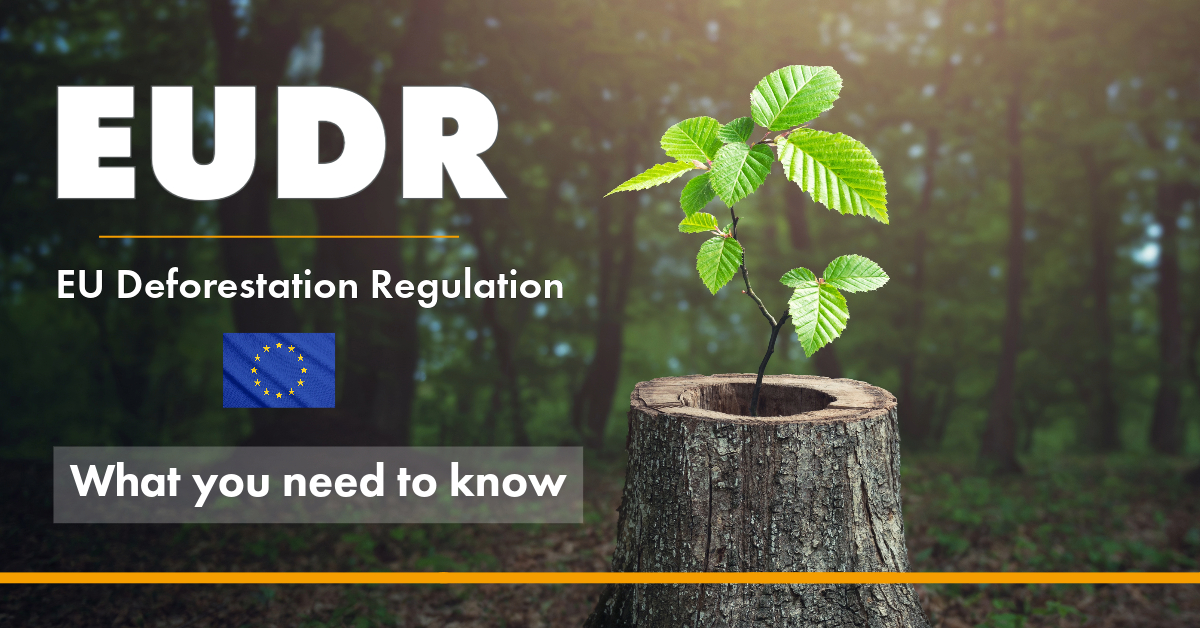
\includegraphics[width=0.6\textwidth]{figs/eudr-europe.jpg}
\end{center}

\begin{itemize}
\item Politique à l'échelle européenne.
\item Consommation en Europe: 10\% de la déforestation mondiale.
\item Les produit issus de la déforestation (cd. huile de palme, viande, soja, café, cacao, bois, caoutchouc) ne pourront plus être importés en Europe.
\end{itemize}
\end{frame}
\begin{frame}[label={sec:org05f8e72}]{Que peut-on faire à notre échelle ?}
\begin{columns}
\begin{column}{0.7\columnwidth}
\begin{itemize}
\item On pourrait penser que les forêts tropicales sont éloignées et qu'on n'a pas de rôle à jouer dans leur protection. Mais plusieurs leviers d'action.
\item Prendre conscience de leur importance pour nos sociétés.
\item Mieux consommer: consommer local et éviter les produits issus de la déforestation. Moins consommer aussi\ldots{}
\item Faire des choix raisonnés le jour où l'on a des responsabilités: banques éthiques, vote sur des programmes appropriés.
\item Beaucoup d'enjeux en France également sur la conservation des écosystèmes (A69, pesticides, loi contre l'artificialisation des sols, etc.).
\end{itemize}
\end{column}
\begin{column}{0.3\columnwidth}
\begin{center}
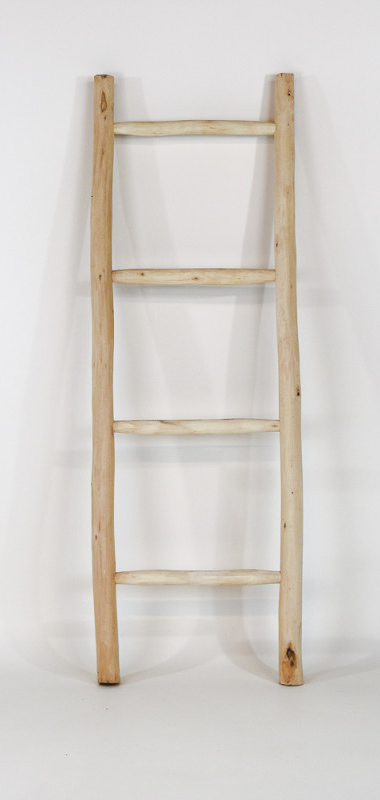
\includegraphics[width=\textwidth]{figs/echelle.jpg}
\end{center}
\end{column}
\end{columns}
\end{frame}
\section{Le métier de chercheur en écologie}
\label{sec:org4ca88d1}

\subsection{Le terrain}
\label{sec:org08cf7f9}

\begin{frame}[label={sec:org58aed0d}]{Le terrain}
\begin{center}
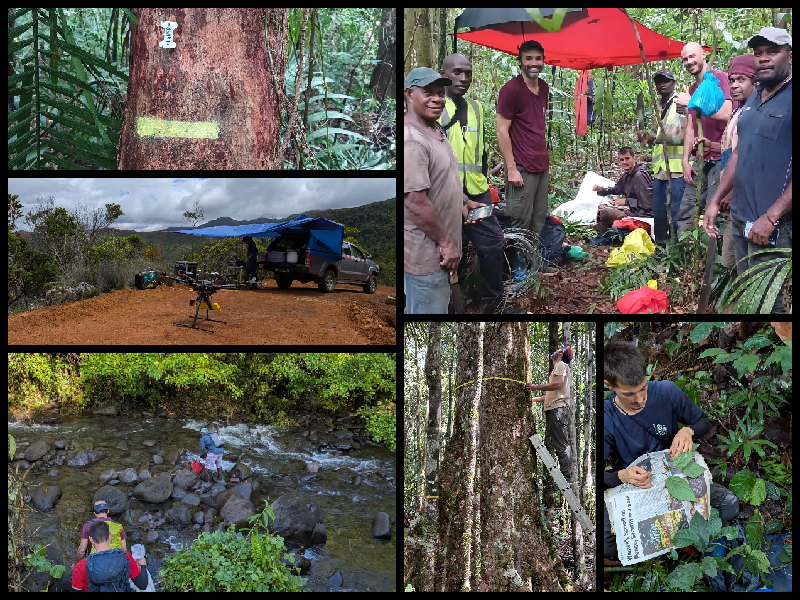
\includegraphics[width=0.6\textwidth]{figs/terrain-collage.png}
\end{center}

\begin{itemize}
\item Mesure des arbres (diamètre, hauteur) et inventaires forestiers.
\item Collecte de spécimens d'herbier, de feuilles, d'échantillon de bois.
\item Survols des forêts par drone-LiDAR.
\item Au moins 1 mois de terrain par an.
\end{itemize}
\end{frame}
\subsection{L'analyse de données}
\label{sec:org0d4efcf}

\begin{frame}[label={sec:org0f1e278}]{L'analyse de données}
\begin{figure}[htbp]
\centering
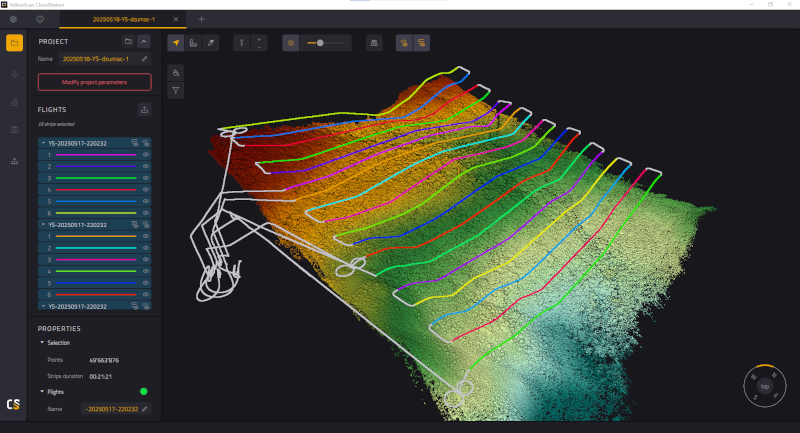
\includegraphics[width=0.7\textwidth]{figs/drone-analyse-de-donnees.png}
\caption{Nuage de points obtenus par drone-lidar au dessus de la forêt calédonienne.}
\end{figure}

\begin{itemize}
\item Beaucoup d'analyses statistiques sur ordinateur.
\item Réalisation de graphiques, de cartes.
\item Programmation de logiciels pour la simulation (code R, Python).
\end{itemize}
\end{frame}
\subsection{Le transfert de connaissances}
\label{sec:org410d966}

\begin{frame}[label={sec:org7937585}]{Le transfert de connaissances}
\begin{center}
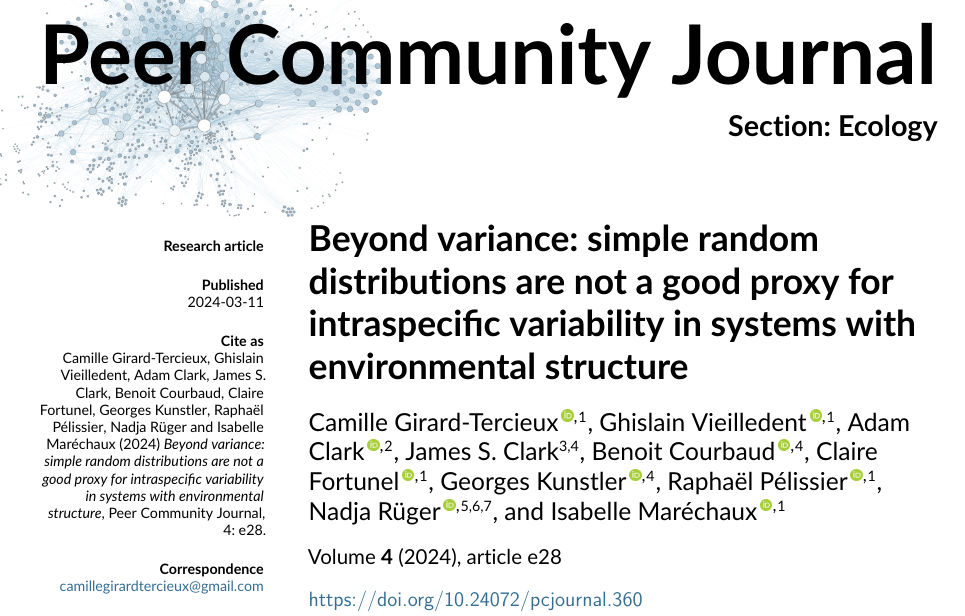
\includegraphics[width=0.6\textwidth]{figs/ecriture-article-scientifique.png}
\end{center}

\begin{itemize}
\item Articles scientifiques.
\item Rapport pour les décideurs.
\item Création d'outils: cartes, logiciels informatique, ex. \url{https://forestatrisk.cirad.fr}.
\item Interaction avec les médias (radio, presse) pour le grand public.
\item Cours aux étudiants.
\end{itemize}
\end{frame}
\subsection{Devenir chercheur}
\label{sec:org3ed86cc}

\begin{frame}[label={sec:org91d71c4}]{Devenir chercheur}
\begin{itemize}
\item A l'école: français (rédaction), math (statistiques), physique (cycle de l'eau et du carbone), biologie (photosynthèse), géographie (cartes), langues étrangères (contexte international), sport (terrain). Toutes ces disciplines sont mobilisées dans le travail de chercheur.
\item Parcours LMD: Plusieurs options pour LM: parcours universitaire ou prépa et école d'ingénieur. Doctorat dans un labo de recherche avec inscription à l'université.
\item Post-doctorats à l'étranger (CDD de chercheur).
\item Concours pour devenir chercheur dans un centre de recherche: ex. CNRS, IRD, INRAe, Cirad, BRGM, CEA, IFREMER, etc.
\item Accessible à tous si on s'en donne les moyens, métier passionnant.
\end{itemize}
\end{frame}
\begin{frame}[label={sec:orgc9880ad}]{En savoir plus}
En savoir plus sur mon métier de chercheur en écologie forestière:

\begin{itemize}
\item \href{https://www.youtube.com/watch?v=4kxdB6Jd4Nw}{Portrait vidéo} par le Cirad.
\item Le site de mon unité de recherche: \href{https://amap.cirad.fr}{UMR AMAP}.
\item Mon \href{https://ecology.ghislainv.fr}{site web} académique.
\end{itemize}
\end{frame}
% %%%%%%%%%%%%%%%%%%%%%%%%%%%%%%%%%%%%%%%%%%%%%%%%%%%%%%%%%%

{
  % Use background image
  \usebackgroundtemplate{%
    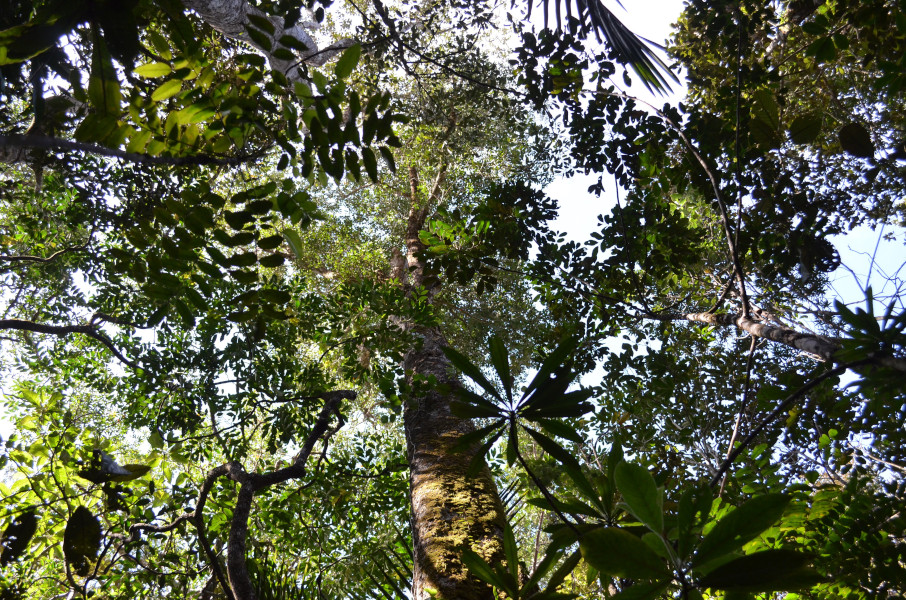
\includegraphics[keepaspectratio=true, height=\paperheight]{figs/Canopy-NC}
  }
  \setbeamertemplate{navigation symbols}{}
  % Remove shadow from block
  \setbeamertemplate{blocks}[rounded][shadow=false]
  \begin{frame}[plain]
  	\vspace*{\stretch{100}} 
    \begin{block}{}
      \begin{center}
        \ldots~Merci pour votre attention~\ldots \\
        \url{https://ecology.ghislainv.fr/presentations.html} \\
        
\includegraphics[width=0.4\textwidth]{figs/partners_logos}
      \end{center}
    \end{block}
  \end{frame}
}
\end{document}
